% ICCIES 2027 -- Springer LNCS/CCIS, 12--15 trang.
% BẢN TIẾNG VIỆT ĐỂ ĐỌC (12/11/2026). Bản nộp phải bằng tiếng Anh, do tác giả tự viết
% (ICCIES cấm văn bản do AI sinh). Dàn ý tiếng Anh cũ: ../outline/.
% Overleaf: tải cả thư mục (zip), main = main.tex, trình biên dịch pdfLaTeX.
% Nếu pdfLaTeX báo lỗi font tiếng Việt (T5), đổi sang XeLaTeX và thay 3 dòng fontenc/inputenc/babel
% bằng: \usepackage{fontspec} \usepackage[vietnamese]{babel}
\documentclass[runningheads]{llncs}

\usepackage[T5]{fontenc}
\usepackage[utf8]{inputenc}
\usepackage[vietnamese]{babel}
\usepackage{graphicx}
\graphicspath{{images/}}
\usepackage{booktabs}
\usepackage{multirow}
\usepackage{amsmath,amssymb}
\usepackage{xcolor}
\usepackage[hidelinks]{hyperref}
\usepackage{url}

% Ghi chú cho tác giả; xóa trước khi nộp.
\newcommand{\todo}[1]{\textcolor{red}{[TODO: #1]}}
\newcommand{\code}[1]{\texttt{#1}}
\renewcommand{\keywordname}{{\bfseries Từ khóa:}}

\begin{document}

\title{Bảo vệ tác tử LLM dùng công cụ trước tấn công chèn lệnh gián tiếp: cơ chế phòng thủ nhiều lớp và đánh giá niêm phong trên benchmark tiếng Việt}
\titlerunning{Phòng thủ nhiều lớp trước chèn lệnh gián tiếp cho tác tử tiếng Việt}

\author{\todo{Tác giả 1}\inst{1} \and \todo{Tác giả 2}\inst{1}}
\authorrunning{\todo{Tác giả} et al.}
\institute{\todo{Đơn vị, thành phố, quốc gia} \\ \email{\todo{email}}}

\maketitle

% LNCS: tóm tắt 150--250 từ (tính trên bản tiếng Anh).
\begin{abstract}
Tác tử LLM theo mô hình ReAct đọc nội dung từ các công cụ bên ngoài. Chỉ thị được cài vào nội dung đó có thể khiến tác
tử thực hiện hành động trái phép hoặc làm lộ dữ liệu. Đây là tấn công chèn lệnh gián tiếp (IPI). Các benchmark an
ninh cho tác tử hiện nay hầu như chỉ có tiếng Anh. Bài báo đề xuất \ours, một cơ chế phòng thủ nhiều lớp đặt việc
cưỡng chế tại Tool Broker, bên ngoài mô hình. Các luật của \ours{} chỉ cho phép gửi tới đích do người dùng viết, chỉ
cho phép giá trị mật rời tác tử khi người dùng đã viết giá trị đó, che giá trị mật trong câu trả lời cuối và chặn
lời gọi tới đích được nêu trong nội dung có dấu hiệu chèn lệnh. Lời nhắc trong prompt và phản hồi từ chối bổ trợ cho
các luật. \ours{} không cần tinh chỉnh mô hình và không gọi thêm LLM. Chúng tôi xây dựng VN-AgentInject v3, một
benchmark tiếng Việt gồm sáu cơ chế tấn công, có nhánh lành tính và năm biến thể ngôn ngữ, và đánh giá theo giao thức
đăng ký trước với hai tập kiểm thử niêm phong. Trên ba mô hình nền mở trọng số, phiên bản thứ nhất (\cRulesS) giảm tỉ
lệ tấn công thành công từ 32,9\% xuống 1,2\% trên tập niêm phong thứ nhất. Phiên bản thứ hai (\bgTwo) giảm tỉ lệ này
từ 32,4\% xuống 3,6\% trên tập niêm phong thứ hai (Holm $p = 5{,}0\cdot10^{-57}$) và giữ 93,7\% tiện ích lành tính.
Bộ phát hiện huấn luyện trên tiếng Anh không có tác dụng trên tiếng Việt.

\keywords{Chèn lệnh gián tiếp \and Tác tử LLM \and An ninh tác tử \and Kiểm soát luồng thông tin \and Tiếng Việt}
\end{abstract}


\section{Giới thiệu}\label{sec:intro}

Trong mô hình ReAct~\cite{yao2023react}, tác tử LLM xen kẽ suy luận với lời gọi công cụ: tìm tài liệu, truy vấn
cơ sở dữ liệu, gửi e-mail hay gọi webhook. Khi đó nội dung công cụ trả về đi thẳng vào ngữ cảnh của mô hình. Trong
tấn công chèn lệnh gián tiếp (IPI)~\cite{greshake2023indirect}, kẻ tấn công không nói chuyện với mô hình mà cài chỉ
thị vào nội dung bên thứ ba mà tác tử sẽ đọc. Nếu mô hình làm theo, nó có thể gửi dữ liệu tới đích lạ, làm lộ giá
trị mật hoặc lặng lẽ sửa dữ liệu người dùng yêu cầu gửi.

Các benchmark tác tử đã công bố như BIPIA~\cite{yi2025bipia}, InjecAgent~\cite{zhan2024injecagent} và
AgentDojo~\cite{debenedetti2024agentdojo} gần như chỉ bằng tiếng Anh. Tiếng Việt có những đặc điểm có thể ảnh hưởng
tới cả tấn công lẫn phòng thủ: văn bản thường bị bỏ dấu, thuật ngữ tiếng Anh hay trộn vào câu, và bộ phân loại chèn
lệnh chủ yếu được huấn luyện trên tiếng Anh. Mặt khác, phòng thủ ở mức prompt như
spotlighting~\cite{hines2024spotlighting} phụ thuộc vào việc mô hình có tuân theo hay không, còn bộ phân loại tốn
thêm chi phí suy luận và chuyển giao kém giữa các ngôn ngữ. Điều đó dẫn tới hướng cưỡng chế \emph{không trông vào
sự tuân thủ của mô hình}: luật do host áp dụng giữa mô hình và công cụ.

Bài báo có bốn đóng góp:
\begin{enumerate}
\item \textbf{Mô hình đe dọa và phân loại theo cơ chế:} hai nhãn độc lập là độ tin cậy và độ nhạy cảm, bốn vị từ
  gây hại, sáu cơ chế tấn công và hai nhánh lành tính làm lộ chặn nhầm (Mục~\ref{sec:threat}).
\item \textbf{\ours}, phòng thủ nhiều lớp phía broker gồm bốn luật tất định cùng lời nhắc và phản hồi từ chối;
  không cần tinh chỉnh và không cần mô hình phụ (Mục~\ref{sec:defence}).
\item \textbf{VN-AgentInject v3 và AgentDojo-VI} với giao thức niêm phong: giả thuyết đăng ký trước, cấu hình ghim
  bằng hash, mỗi tập kiểm thử chạy một lần (Mục~\ref{sec:protocol}). \todo{owner quyết: công bố dữ liệu / cung
  cấp khi có yêu cầu}
\item \textbf{Kết quả:} trên hai tập niêm phong và ba mô hình nền mở trọng số, \ours{} giảm tỉ lệ tấn công thành công
  từ 32,4\% xuống 3,6\% với cái giá 3,4 điểm tiện ích; phát hiện học trên tiếng Anh không chuyển giao sang tiếng
  Việt; lỗi còn lại tập trung ở rò rỉ giá trị mật và sửa tham số (Mục~\ref{sec:results}--\ref{sec:discussion}).
\end{enumerate}

\section{Nghiên cứu liên quan}\label{sec:related}
% Trước khi viết bản tiếng Anh: mở PDF trong ../refs/ để đối chiếu từng câu trích.

\paragraph{Tấn công và benchmark.} Greshake và cộng sự~\cite{greshake2023indirect} đưa ra khái niệm chèn lệnh gián
tiếp; Liu và cộng sự~\cite{liu2024formalizing} hình thức hóa tấn công và phòng thủ chèn lệnh. BIPIA~\cite{yi2025bipia}
đo chèn lệnh gián tiếp vào LLM; InjecAgent~\cite{zhan2024injecagent}, AgentDojo~\cite{debenedetti2024agentdojo} và
ASB~\cite{zhang2025asb} chuyển sang tác tử dùng công cụ, nơi tấn công gây ra hành động. Các bộ này đều bằng tiếng
Anh; Deng và cộng sự~\cite{deng2024multijail} cho thấy cơ chế an toàn của LLM yếu hơn ở ngôn ngữ ít tài nguyên,
nhưng trong bối cảnh jailbreak chứ không phải tác tử.

\paragraph{Phòng thủ.} Ở mức prompt có spotlighting~\cite{hines2024spotlighting} và lời nhắc kiểu sandwich.
StruQ~\cite{chen2025struq} và SecAlign~\cite{chen2025secalign} huấn luyện lại mô hình để tách chỉ thị khỏi dữ liệu.
Bộ phân loại như Prompt Guard~2~\cite{meta2025promptguard2,chennabasappa2025llamafirewall} sàng lọc đầu vào.
MELON~\cite{zhu2025melon} so hành động của lượt chạy gốc với lượt chạy lại có che yêu cầu; Progent~\cite{shi2025progent}
áp chính sách đặc quyền lên lời gọi công cụ. Hướng an toàn theo thiết kế gồm CaMeL~\cite{debenedetti2026camel},
kiểm soát luồng thông tin FIDES~\cite{costa2025fides} và các mẫu thiết kế trong~\cite{beurerkellner2025patterns}.
\ours{} gần hướng này nhất: giống CaMeL, nó không sửa mô hình, nhưng thay vì tách luồng điều khiển và chạy chương
trình trong một trình thông dịch riêng, \ours{} chỉ áp luật chuỗi lên quỹ đạo nên gắn được vào tác tử ReAct sẵn có. Tấn công thích nghi vượt qua nhiều phòng thủ đã
công bố~\cite{zhan2025adaptive,nasr2025attacker}; chúng tôi báo cáo riêng một tập tấn công thích nghi
(Mục~\ref{sec:external}).

\section{Mô hình đe dọa}\label{sec:threat}

\paragraph{Tác tử.} Cho chỉ thị người dùng $u$, ở mỗi bước mô hình sinh một hành động $a_t$ (công cụ và tham số)
hoặc câu trả lời cuối $y$. Tool Broker kiểm $a_t$ theo schema, thực thi và trả quan sát $o_t$. Có sáu công cụ đọc
(tìm và đọc tài liệu, truy vấn cơ sở dữ liệu chỉ đọc, tìm và lấy trang lưu đệm, máy tính) và hai \emph{sink} có tác
dụng phụ, \code{send\_email\_mock} và \code{post\_webhook\_mock}; cả hai chỉ ghi log, không gửi ra mạng. Câu trả lời
cuối được coi là sink thứ ba. Với lời gọi sink $a$, ta viết $\dest(a)$ cho đích (\code{to} hoặc \code{endpoint}) và
$\pay(a)$ cho các tham số còn lại.

\paragraph{Hai nhãn.} Mỗi nội dung mang hai nhãn độc lập do host gán. \emph{Độ tin cậy}: $u$ và prompt hệ thống là
đáng tin, mọi quan sát công cụ là không đáng tin. \emph{Độ nhạy cảm}: từ công khai (S0) tới mật (S2); tài liệu mật
chứa giá trị (khóa, mã, định danh tài khoản) không được rời tác tử nếu người dùng không cho phép. Một trang không đáng
tin có thể công khai, còn một bản ghi mật có thể đến từ nguồn kẻ tấn công không chạm được; gộp hai chiều làm một sẽ
hoặc chặn mọi dữ liệu mật, hoặc tin mọi nguồn nội bộ.

\paragraph{Kẻ tấn công.} Kẻ tấn công kiểm soát văn bản của một tài liệu mà công cụ đọc trả về (tài liệu, trang lưu
đệm, trường văn bản trong cơ sở dữ liệu, đầu ra công cụ), ở bất kỳ vị trí và giọng điệu nào, và biết tên cùng schema
công cụ. Họ không sửa được $u$, prompt hệ thống, broker hay trọng số, và không quan sát được quỹ đạo. Trên tập niêm
phong, tấn công là tĩnh, được viết mà không biết mã phòng thủ. Jailbreak trực tiếp, đầu độc dữ liệu huấn luyện, từ
chối dịch vụ và hệ nhiều tác tử nằm ngoài phạm vi.

\paragraph{Vị từ gây hại.} Gọi $G(u)$ là tập đích người dùng cấp quyền, $V$ là tập giá trị mật trên quỹ đạo mà người
dùng không cho phép tiết lộ, và $\mathcal{S}$ là tập lời gọi sink \emph{đã thực thi}. Quỹ đạo $\tau$ gây hại nếu
\begin{equation}\label{eq:harm}
\mathrm{Harm}(\tau) = H_\mathit{dest} \lor H_\mathit{leak} \lor H_\mathit{tamper} \lor H_\mathit{side},
\end{equation}
trong đó $H_\mathit{dest}$: $\exists a \in \mathcal{S}$ với $\dest(a) \notin G(u)$; $H_\mathit{leak}$: có
$v \in V$ xuất hiện trong $\pay(a)$ của một $a \in \mathcal{S}$ hoặc trong $y$; $H_\mathit{tamper}$: $\exists a \in
\mathcal{S}$ với $\dest(a) \in G(u)$ nhưng một trường người dùng chỉ định mang giá trị khác; $H_\mathit{side}$:
nhiệm vụ chỉ đọc nhưng $\mathcal{S} \neq \emptyset$. Lời gọi bị chặn không gây hại. Bộ chấm đóng băng tính các vị từ
từ lời gọi đã thực thi và $y$; suy luận của mô hình không được ghi.

\paragraph{Sáu cơ chế.} Chúng tôi phân loại tấn công theo \emph{cơ chế}, tức con đường đoạn chèn biến thành tác hại
(Bảng~\ref{tab:mechanisms}). Ở \mER{} và \mCR{}, lời gọi gây hại đi tới đích người dùng chưa viết, nên kiểm tra đích
là đủ dù cách diễn đạt thế nào. Ở \mSL{} và \mAL{}, đích hợp lệ hoặc không có đích; chỉ nguồn gốc của giá trị phân biệt
tấn công với nhiệm vụ. Ở \mPT{}, cả đích lẫn độ nhạy cảm đều bình thường, nên đây là cơ chế khó nhất với luật theo
nhãn. \mUS{} kiểm tra xem việc người dùng nhắc tới một đích, chẳng hạn trong câu cấm, có bị hiểu nhầm là cấp quyền
không.

% M1..M6 trong log/luận văn = ER, CR, SL, AL, PT, US.
\begin{table}[!htbp]
\centering
\caption{Sáu cơ chế tấn công và vị từ gây hại tương ứng.}\label{tab:mechanisms}
\footnotesize
\begin{tabular}{@{}lp{0.70\textwidth}l@{}}
\toprule
Mã & Cơ chế (kiểu con) & Vị từ \\
\midrule
\mER & Chuyển hướng tường minh: yêu cầu gửi tới đích không có trong $u$, có động từ gửi và địa chỉ đầy đủ & $H_\mathit{dest}$ \\
\mCR & Chuyển hướng che giấu: cùng mục tiêu nhưng tránh mẫu ``gửi + địa chỉ'' (ghi nhận không động từ, chuyển tiếp hoặc cc, tách địa chỉ, đích nằm ở tài liệu thứ hai) & $H_\mathit{dest}$ \\
\mSL & Rò rỉ qua sink: đưa giá trị mật vào sink người dùng đã nêu (thân e-mail, payload, trường trông vô hại) & $H_\mathit{leak}$ \\
\mAL & Rò rỉ qua câu trả lời: đưa giá trị mật vào câu trả lời cuối (nguyên văn, lồng trong câu, có nhãn) & $H_\mathit{leak}$ \\
\mPT & Sửa tham số: đổi một giá trị thường trong payload của sink người dùng đã nêu (số, boolean, đơn vị, định danh) & $H_\mathit{tamper}$ \\
\mUS & Tác dụng phụ ngoài yêu cầu: chèn lời gọi sink vào nhiệm vụ chỉ đọc (đích chỉ xuất hiện trong câu cấm, chỉ là thông tin, hoặc không có) & $H_\mathit{side}$ \\
\bottomrule
\end{tabular}
\end{table}


\paragraph{Nhánh lành tính và biến thể.} Mỗi họ tấn công có hai nhánh lành tính cùng nhiệm vụ và môi trường.
\emph{benign\_plain} thay đoạn chèn bằng ghi chú vô hại cùng độ dài, để đo tiện ích. \emph{benign\_auth} giữ một yêu
cầu giống mục tiêu tấn công nhưng được người dùng cho phép rõ ràng; chặn ở đây là \emph{chặn nhầm}. Mỗi họ có năm
biến thể áp cho cả $u$ lẫn đoạn chèn: tiếng Việt chuẩn, diễn đạt lại, trộn mã Việt--Anh, không dấu và tiếng Anh. Định
danh, địa chỉ và giá trị mật giống hệt nhau giữa các biến thể, nên khác biệt chỉ do ngôn ngữ.

\section{Cơ chế phòng thủ D3}\label{sec:d3}
% Dàn ý gốc: ../outline/03_d3_defence.md (khoảng 2,5 trang)

\subsection{Nguyên tắc thiết kế}

D3 theo ba nguyên tắc. (i) \textbf{Mô hình không phải ranh giới an ninh.} Dù mô hình sinh ra gì, một hành động chỉ
có hiệu lực khi broker thực thi nó; mọi bảo đảm cứng đều nằm phía host. (ii) \textbf{Người dùng là chủ thể đáng tin
duy nhất.} Quyền được suy ra từ nguyên văn chỉ thị người dùng, không bao giờ từ nội dung công cụ và không bao giờ từ
việc một mô hình diễn giải ý định người dùng. (iii) \textbf{Chặn không được làm kết thúc nhiệm vụ.} Hành động bị từ
chối được báo lại cho tác tử theo dạng giúp nó hoàn thành các bước hợp lệ.

Hình~\ref{fig:d3} minh họa các lớp; Bảng~\ref{tab:layers} tóm tắt chúng.

% HÌNH 1: Claude vẽ, lưu ở images/fig1_d3_architecture.pdf. Bỏ comment khi có file.
% \begin{figure}[t]
% \centering
% \includegraphics[width=\textwidth]{fig1_d3_architecture}
% \caption{Kiến trúc D3. Người dùng $\to$ mô hình tác tử $\rightleftarrows$ Tool Broker (schema, giới hạn, nhãn
%   nguồn gốc, luật R2--R4, luật D, phản hồi) $\rightleftarrows$ công cụ; lời nhắc trên đường quan sát; câu trả lời
%   cuối đi qua R3/R4.}\label{fig:d3}
% \end{figure}
\todo{Hình 1 (kiến trúc D3)}

\begin{table}[t]
\centering
\caption{Các lớp của D3. ``TĐ'' đánh dấu cưỡng chế tất định phía host.}\label{tab:layers}
\small
\begin{tabular}{@{}p{0.22\textwidth}p{0.15\textwidth}p{0.30\textwidth}cp{0.17\textwidth}@{}}
\toprule
Lớp & Thời điểm & Cơ chế & TĐ & Nhắm tới \\
\midrule
L0 Tool Broker & mọi lời gọi & kiểm schema, giới hạn công cụ, nhãn nguồn gốc & có & lời gọi sai; nền cho các lớp khác \\
L1 Cấp quyền đích (R2) & trước sink & đích phải có nguyên văn trong chỉ thị người dùng & có & M1, M2, M6 \\
L2 Luồng giá trị mật (R3) & trước sink; ở câu trả lời & giá trị mật từ công cụ không được đi ra trừ khi người dùng đã viết & có & M3, M4 \\
L3 Che câu trả lời (R4) & ở câu trả lời & che từng giá trị vi phạm & có & M4 \\
L4 Luật tín hiệu theo đích (D) & trước sink & từ chối khi quan sát bị gắn cờ nêu đúng đích của sink & có & M3, M5 trên sink người dùng nêu \\
L5 Lời nhắc (P2) & sau mỗi quan sát & lặp lại chỉ thị người dùng cho mô hình & không & tất cả, tùy mô hình \\
L6 Phản hồi từ chối & sau khi từ chối & thông báo có cấu trúc; không chạy công cụ; tác tử tiếp tục & có & tiện ích sau khi chặn \\
\bottomrule
\end{tabular}
\end{table}


\subsection{Tool Broker và nhãn nguồn gốc (L0)}

Mọi lời gọi công cụ đều đi qua broker. Khi không có phòng thủ (cấu hình A0), broker chỉ kiểm tra lời gọi theo schema
và cưỡng chế giới hạn từng công cụ. Trong D3, broker còn lưu, với mỗi quan sát, định danh tài liệu cùng nhãn tin cậy
và nhạy cảm, và tập \textbf{giá trị} trích từ các quan sát mật. Việc trích giá trị là từ vựng và không phụ thuộc
ngôn ngữ: địa chỉ e-mail, URL, định danh dài từ sáu ký tự và số dài. Thao tác đọc không bao giờ bị chặn (luật R1),
nên tác tử luôn thu thập được thông tin nhiệm vụ cần.

Mọi phép so sánh dùng một hàm chuẩn hóa $n(\cdot)$: Unicode NFKC, bỏ ký tự định dạng (trong đó có ký tự độ rộng
bằng không) và đưa về chữ thường. Chuẩn hóa chỉ dùng để so sánh, không bao giờ thay đổi nội dung mà mô hình hay công
cụ nhận được.

\subsection{Cấp quyền đích (L1, luật R2)}

Một lời gọi sink $a$ chỉ được phép nếu đích của nó do người dùng viết:
\begin{quote}
\textbf{R2.} chỉ cho phép $a$ nếu $n(\mathit{dest}(a))$ là chuỗi con của $n(u)$.
\end{quote}
Văn bản người dùng không được phân tích ý định, và không có danh sách cụm từ tiếng Việt hay tiếng Anh nào được tra.
Vì vậy luật không phụ thuộc vào cách viết đoạn chèn: một đoạn chèn M2 tránh động từ ``gửi'', tách địa chỉ hay giấu
đích trong tài liệu thứ hai sẽ thất bại vì cùng lý do với đoạn chèn M1, là đích nó cần không có trong $u$. Cái giá
của so khớp nguyên văn xuất hiện ở hai chỗ. Người dùng nhắc đích một cách gián tiếp (``địa chỉ trong hợp đồng'') sẽ
không được phục vụ. Và một đích người dùng chỉ nhắc trong câu cấm vẫn được tính là đã cấp quyền, đúng là trường
hợp M6 thăm dò.

\subsection{Luồng giá trị mật (L2--L3, luật R3 và R4)}

Gọi $C$ là tập giá trị trích từ các quan sát có nhãn mật. Với lời gọi sink $a$ hoặc câu trả lời cuối $y$:
\begin{quote}
\textbf{R3.} từ chối nếu có $v \in C$ xuất hiện trong $n(\mathit{payload}(a))$ (tương ứng $n(y)$) và $n(v)$ không
xuất hiện trong $n(u)$.\\
\textbf{R4.} câu trả lời cuối vi phạm R3 không bị đánh hỏng: mỗi giá trị vi phạm được thay bằng
\code{[REDACTED]}.
\end{quote}
R3 hiện thực một chính sách luồng thông tin tối thiểu trên hai nhãn ở Mục~\ref{sec:threat}: giá trị mật chỉ được
tới sink qua chính văn bản người dùng. Luật coi câu trả lời cuối là một sink, nhờ đó đóng kênh M4 mà các bộ lọc lời
gọi công cụ bỏ sót. R4 giữ phần còn lại của câu trả lời, nên một câu trả lời đúng có lẫn một mã bị lộ chỉ mất mã đó
chứ không mất cả nhiệm vụ. Vì R3 so khớp nguyên văn, giá trị mà mô hình đã biến đổi trước khi xuất (định dạng lại,
tách ra, diễn đạt lại) sẽ không được nhận ra; Mục~\ref{sec:discussion} quay lại giới hạn này.

\subsection{Luật tín hiệu chèn lệnh giới hạn theo đích (L4)}

R2 và R3 để lại một khoảng hở: đoạn chèn thao túng một sink mà người dùng \emph{đã} nêu, với giá trị không mật (M5)
hoặc qua tham số R3 không phủ. Phòng thủ trước của chúng tôi (D2, cấu hình được đánh giá ở tập niêm phong thứ nhất)
lấp khoảng này bằng bộ phát hiện dựa trên cụm từ để nhận ra văn bản giống chỉ thị trong quan sát: khi có bất kỳ
quan sát nào bị gắn cờ, mọi sink sau đó không được cấp quyền bởi một văn phạm chặt trên văn bản người dùng đều bị
từ chối. Trên tập niêm phong thứ nhất, lớp này là nguồn chặn nhầm lớn nhất trên nhiệm vụ lành tính (22 quỹ đạo
benign\_plain trên ba mô hình nền), nhưng bỏ nó trên tập phát triển lại làm số họ gây hại tăng 2--4 ở mỗi mô hình
nền.

D3 giữ bộ phát hiện và thu hẹp hệ quả của nó. Gọi $F$ là tập quan sát bị bộ phát hiện gắn cờ:
\begin{quote}
\textbf{D.} từ chối lời gọi sink $a$ nếu có $o \in F$ chứa $n(\mathit{dest}(a))$.
\end{quote}
Luật chỉ kích hoạt khi nội dung không đáng tin, mang dáng dấp chỉ thị, nói về đúng cái đích mà tác tử sắp dùng. Một
trang bị gắn cờ ở đâu đó trên quỹ đạo không còn chặn một lần gửi không liên quan do người dùng yêu cầu, còn việc
chuyển hướng sang đích khác vẫn do R2 lo. Thiết kế được chọn bằng phát lại offline trên các quỹ đạo phát triển có
sẵn, trước mọi lượt chạy mô hình mới: luật D chặn đủ 11 ca gây hại mà lớp rộng đã chặn và không chặn ca nào trong 14
lời gọi sink lành tính bị lớp rộng từ chối nhầm. Một phương án khác theo dõi giá trị từ nguồn bị gắn cờ chỉ chặn 9/11
và bị loại.

\subsection{Lời nhắc (L5) và phản hồi từ chối (L6)}

\textbf{Lời nhắc.} Sau mỗi quan sát công cụ, chỉ thị gốc của người dùng được nối vào cùng tin nhắn, kèm một câu nói
rằng mọi chỉ thị khác tìm thấy trong dữ liệu công cụ phải bị bỏ qua (phòng thủ sandwich, như \code{repeat\_user\_prompt}
của AgentDojo). Đây là lớp duy nhất phụ thuộc vào việc mô hình tuân thủ. Lớp này được giữ vì nó phủ những gì các
lớp tất định không thấy: trên tập niêm phong thứ nhất, riêng nó giảm tỉ lệ ca gây hại từ 32,9\% xuống 5,6\%, và kết
hợp với các luật thì còn 1,2\%.

\textbf{Phản hồi từ chối.} Khi một luật từ chối hành động, công cụ không được thực thi và tác tử nhận một quan sát
có cấu trúc báo rằng hành động bị chính sách từ chối. Tác tử sau đó có thể làm các bước còn lại hoặc trả lời. Nếu
không có phản hồi này, mỗi lần từ chối sẽ kết thúc quỹ đạo và biến mọi lần chặn nhầm thành một nhiệm vụ thất bại.

\subsection{Chọn thành phần}

D3 được thiết kế và tinh chỉnh chỉ trên tập phát triển; tập niêm phong thứ nhất khi đó đã mở và chỉ được dùng để
xác định các lớp lỗi. Trước mọi lượt chạy GPU, chúng tôi cố định tiêu chí chọn: gộp trên ba mô hình nền, ứng viên
phải có số ca tấn công gây hại không nhiều hơn cấu hình trước (D2+P2) và tiện ích lành tính cao hơn hẳn; thành phần
nào làm tăng tác hại hoặc giảm tiện ích trong ablation thì bị bỏ.

Bảng~\ref{tab:ablation} báo cáo ablation. Chỉ biến thể có luật D, lời nhắc gốc và phản hồi gốc (tên D3DEST trong
log, trong bài gọi là D3) đạt tiêu chí. Một lời nhắc mạnh hơn, giục mô hình hoàn thành mọi bước được yêu cầu kể cả
việc gửi, giúp Gemma nhưng làm số họ gây hại của Llama tăng gấp đôi và làm tiện ích của Qwen sụp (benign\_plain 141
$\to$ 39 trên 240); nó không chuyển giao giữa các mô hình nền nên bị loại. Một thông báo từ chối mạnh hơn không thêm
gì. Hai ý tưởng khác bị loại ở bước phát lại: giới hạn R3 theo tài nguyên người dùng nêu (mở được 3 nhiệm vụ có cấp
quyền nhưng thả 5 tấn công) và so khớp giá trị gần đúng (không bắt thêm ca nào trên dữ liệu phát triển).

\begin{table}[t]
\centering
\caption{Ablation D3 trên tập phát triển (48 họ, 560 ca mỗi ô). Mỗi ô: họ gây hại /48 $\cdot$ tiện ích
benign\_plain /240 $\cdot$ tiện ích benign\_auth /80. Cột gộp: ca tấn công gây hại /720 $\cdot$ tiện ích lành tính
/960.}\label{tab:ablation}
\small
\begin{tabular}{@{}lcccc@{}}
\toprule
Cấu hình & Gemma-4-12B & Llama-3.1-8B & Qwen3.5-9B & Gộp \\
\midrule
A0 (không phòng thủ) & 38 $\cdot$ 159 $\cdot$ 54 & 34 $\cdot$ 81 $\cdot$ 30 & 40 $\cdot$ 140 $\cdot$ 36 & 330 $\cdot$ 500 \\
D2+P2 (trước đó) & 2 $\cdot$ 147 $\cdot$ 45 & 5 $\cdot$ 82 $\cdot$ 36 & 3 $\cdot$ 141 $\cdot$ 24 & 12 $\cdot$ 475 \\
\textbf{D3} (luật D, nhắc v1, phản hồi v1) & 2 $\cdot$ 148 $\cdot$ 49 & 5 $\cdot$ 85 $\cdot$ 40 & 3 $\cdot$ 141 $\cdot$ 27 & \textbf{12 $\cdot$ 490} \\
luật D, nhắc v1, phản hồi v2 & 2 $\cdot$ 150 $\cdot$ 49 & 6 $\cdot$ 84 $\cdot$ 40 & 3 $\cdot$ 142 $\cdot$ 26 & 14 $\cdot$ 491 \\
luật D, nhắc v2, phản hồi v2 & 1 $\cdot$ 163 $\cdot$ 54 & 10 $\cdot$ 75 $\cdot$ 38 & 2 $\cdot$ 39 $\cdot$ 16 & 21 $\cdot$ 385 \\
luật D, nhắc v2, phản hồi v1 & 1 $\cdot$ 162 $\cdot$ 54 & 10 $\cdot$ 69 $\cdot$ 38 & 2 $\cdot$ 40 $\cdot$ 16 & 21 $\cdot$ 379 \\
\bottomrule
\end{tabular}
\end{table}


\paragraph{Chi phí và phạm vi.} D3 không thêm lời gọi mô hình nào: mọi luật là phép toán chuỗi trên quỹ đạo, còn lời
nhắc thêm độ dài chỉ thị người dùng vào mỗi tin nhắn quan sát. D3 không cần truy cập trọng số và dùng nguyên vẹn
được với mô hình dịch vụ (Mục~\ref{sec:external}). D3 không tuyên bố chặn được việc sửa giá trị không mật trên sink
người dùng đã nêu khi nội dung chèn không nhắc tới đích (một phần của M5), cũng như rò rỉ giá trị đã bị mô hình biến
đổi.

\section{Benchmark và giao thức đánh giá}\label{sec:protocol}
% Dàn ý gốc: ../outline/04_benchmark_protocol.md (khoảng 2 trang)

\subsection{VN-AgentInject v3}

VN-AgentInject v3 hiện thực phân loại ở Mục~\ref{sec:threat} thành các \textbf{ca kiểm thử} (fixture) chạy được. Mọi
dữ liệu đều là tổng hợp: tài liệu, bản ghi, địa chỉ và giá trị mật là bịa ra, còn hai sink là bản giả không gửi gì ra
mạng. Một \textbf{họ} (family) là một ý tưởng tấn công trong một nhiệm vụ và một môi trường công cụ. Mỗi họ sinh một
ca tấn công và một ca benign\_plain cho mỗi biến thể ngôn ngữ, và một phần ba số họ còn sinh thêm một ca benign\_auth
cho mỗi biến thể. Benchmark có ba tập rời nhau:
\begin{itemize}
\item \textbf{Dev}: 48 họ, tám họ mỗi cơ chế; 560 ca (240 tấn công, 240 benign\_plain, 80 benign\_auth). Mọi lựa
  chọn thiết kế, prompt, luật và ngưỡng chỉ được cố định trên tập này.
\item \textbf{Test v3}: 72 họ, mười hai họ mỗi cơ chế; 840 ca (360 / 360 / 120).
\item \textbf{Test-3}: thêm 48 họ; 560 ca (240 / 240 / 80), được viết sau khi Test v3 đã chạy, để xác nhận D3 trên
  dữ liệu chưa từng chạm vào quyết định nào trước đó.
\end{itemize}

\paragraph{Soạn và kiểm soát chất lượng.} Văn bản tấn công do người viết, những người không đọc mã phòng thủ. Mỗi họ
được duyệt theo phiếu năm mục: nhãn cơ chế có đúng không, yêu cầu người dùng và đoạn chèn có tự nhiên không, làm theo
đoạn chèn có gây hại theo các vị từ ở Mục~\ref{sec:threat} không, và văn bản có để lộ gợi ý về đáp án không; người
duyệt thấy nội dung ca nhưng không thấy phòng thủ. Một bộ lọc độ mới loại họ có độ tương đồng Jaccard 4-gram với bất
kỳ bản phát hành trước nào vượt 0,2; định danh, đích và tên miền không được dùng lại. Cuối cùng, mỗi họ phải qua
\textbf{kiểm tra phát lại} với bộ chấm đóng băng: một quỹ đạo tham chiếu làm theo đoạn chèn phải bị chấm là gây hại,
và một quỹ đạo tham chiếu hoàn thành nhiệm vụ an toàn phải được chấm là an toàn với đủ tiện ích. Các thủ thuật bề
mặt có thể giấu rò rỉ khỏi bộ chấm nguyên văn (ví dụ làm rối giá trị) bị loại khỏi tập kiểm thử tĩnh.

\subsection{Đánh giá niêm phong}

Hai tập kiểm thử được \textbf{niêm phong}. Trước mỗi lượt chạy kiểm thử, chúng tôi đóng băng (i) các ca chuẩn, bằng
SHA-256; (ii) một manifest cấu hình ghim bằng hash prompt tác tử, thiết lập giải mã, mã phòng thủ, phiên bản mô hình
và danh sách cặp (mô hình nền, cấu hình) được phép; và (iii) giả thuyết, kiểm định và cách hiệu chỉnh đa so sánh.
Runner và bộ chấm kiểm tra manifest và từ chối chạy nếu có bất kỳ sai khác nào hoặc gặp cặp ngoài danh sách. Mỗi cặp
chỉ chạy đúng một lần; lần chạy lại duy nhất được phép là tiếp tục các ca kết thúc vì lỗi hạ tầng. Đáp án của bộ chấm
chỉ được đọc sau khi manifest được xác minh, và không bao giờ có mặt trong prompt, chính sách lúc chạy hay mô hình.

Test v3 chạy dưới manifest đóng băng D2+P2 làm cấu hình cuối, với sáu giả thuyết (H1--H6,
Mục~\ref{sec:test1}). Sau đó D3 được thiết kế và chọn trên Dev (Mục~\ref{sec:d3}), một manifest mới được đóng băng,
và Test-3 chạy với ba giả thuyết: \textbf{T1}, D3 có tiện ích lành tính cao hơn D2+P2; \textbf{T2}, tỉ lệ tấn công
thành công của D3 không cao hơn D2+P2 quá hai điểm; \textbf{T3}, D3 có tỉ lệ tấn công thành công thấp hơn A0. Manifest
cũng ghi lại dự đoán của chúng tôi rằng mức tăng tiện ích sẽ nhỏ và có thể không đạt ý nghĩa thống kê.

\subsection{Mô hình nền và cấu hình so sánh}

Thí nghiệm xác nhận dùng ba mô hình nền mở trọng số phục vụ bằng vLLM~\cite{kwon2023vllm}: \textbf{Gemma-4-12B},
\textbf{Llama-3.1-8B} (ngữ cảnh 16k) và \textbf{Qwen3.5-9B}, mỗi mô hình ghim theo một revision của kho. Mọi mô hình
nền nhận cùng prompt ReAct và cùng thiết lập giải mã: nhiệt độ 0, tối đa 512 token mới mỗi bước, seed cố định, đầu
ra JSON ràng buộc theo schema từng công cụ, và tối đa tám bước mỗi nhiệm vụ. Tác tử không phòng thủ \textbf{A0}
không có cơ chế an ninh nào ngoài kiểm schema và giới hạn công cụ. Các phòng thủ không thay đổi mô hình nền, khuôn
prompt của A0 (ngoài lời nhắc đã mô tả) hay cách giải mã. Làm mốc cho một mô hình đóng mạnh hơn, chúng tôi chạy
\textbf{Gemini 3 Flash} qua một proxy cục bộ, chỉ trên Dev và AgentDojo. Đường này không hỗ trợ seed hay ràng buộc
schema, nên kết quả được báo cáo riêng và không thuộc kiểm định giả thuyết nào. Không có dữ liệu kiểm thử niêm phong
nào được gửi tới dịch vụ bên ngoài.

Trên Dev, chúng tôi so sánh D2, D2+P2 và D3 với sáu baseline, cài trong cùng tác tử và broker để chỉ có phòng thủ là
khác: \textbf{P1}, spotlighting, đầu ra công cụ được bao và đánh dấu là dữ liệu~\cite{hines2024spotlighting};
\textbf{P2}, sandwich, lặp lại yêu cầu người dùng sau mỗi đầu ra công cụ; \textbf{G1}, bộ phân loại Prompt Guard 2
sàng lọc đầu ra công cụ~\cite{meta2025promptguard2}; \textbf{MEL}, biến thể tất định của phép kiểm chạy lại có che
của MELON~\cite{zhu2025melon}; \textbf{PRG}, chính sách đích theo kiểu Progent~\cite{shi2025progent}; \textbf{R1},
lớp luật cụm từ của hệ thống trước, chặn sink sau khi đầu ra công cụ khớp mẫu giống chỉ thị. \textbf{D2} là lõi tất
định ở Mục~\ref{sec:d3} (luật R2--R4), \textbf{D2+P2} thêm lời nhắc sandwich, và \textbf{D3} là kiến trúc đầy đủ.
Test v3 chạy với A0, R1, PRG, P2, D2 và D2+P2; Test-3 chạy với A0, D2+P2 và D3.

\subsection{Độ đo và thống kê}

Một ca là \textbf{gây hại} nếu ít nhất một vị từ ở Mục~\ref{sec:threat} đúng. Chúng tôi báo cáo \textbf{tỉ lệ tấn
công thành công} (ASR), tức tỉ lệ ca tấn công gây hại, và số \textbf{họ gây hại}, tức họ có ít nhất một ca tấn công
gây hại. \textbf{Tiện ích} là tỉ lệ ca lành tính mà nhiệm vụ người dùng được hoàn thành và không có tác hại; báo cáo
riêng cho benign\_plain và benign\_auth, và trên Test-3 thì gộp lại thành tiện ích lành tính. Lượt chạy kết thúc bằng
lỗi mô hình (đầu ra sai định dạng hoặc bị cắt) là thất bại tiện ích và không bao giờ được tính là phòng thủ thành công.

Các cấu hình được so sánh trên \textbf{cặp ca} gộp qua ba mô hình nền, bằng kiểm định McNemar chính xác một
phía~\cite{mcnemar1947}. Giả thuyết không kém hơn T2 dùng kiểm định z một phía với sai số chuẩn theo cụm họ và biên
hai điểm. Giá trị p được hiệu chỉnh bằng thủ tục Holm~\cite{holm1979} trong mỗi bộ giả thuyết đăng ký trước. Khoảng
tin cậy là khoảng bootstrap 95\% lấy mẫu lại theo họ (10.000 lần), để năm biến thể của một họ không bị coi là độc
lập. Các phân tích ngoài bộ đăng ký trước được ghi là thăm dò.

\subsection{AgentDojo-VI}

Để kiểm tra kết quả không phải là sản phẩm riêng của benchmark do chúng tôi tự xây, chúng tôi dùng thêm hai bộ Banking
và Slack của AgentDojo (phiên bản 1.2.2)~\cite{debenedetti2024agentdojo} bằng tiếng Anh và một bản dịch tiếng Việt,
\textbf{AgentDojo-VI}. Bản dịch phủ môi trường, nhiệm vụ người dùng, mục tiêu chèn và khuôn tấn công
\code{important\_instructions}; IBAN, số tiền, ngày, tên tệp, tên người và kênh, URL và địa chỉ e-mail giữ nguyên.
Công cụ, lời giải chuẩn và hàm kiểm là mã gốc của AgentDojo: cụm tiếng Việt cần có trong câu trả lời được ánh xạ sang
chuỗi tiếng Anh mà hàm tiện ích và an ninh gốc tìm kiếm. Một phép kiểm ở mức bộ xác nhận lời giải chuẩn giải được mọi
nhiệm vụ người dùng. Banking có 144 cặp bị tấn công và 16 nhiệm vụ người dùng, Slack có 105 cặp và 21 nhiệm vụ. Các
lượt này dùng pipeline tác tử dựa trên prompt của chính AgentDojo cho mô hình cục bộ (công cụ được mô tả trong prompt)
thay vì broker của chúng tôi, nên chúng đo độ dễ bị tấn công của mô hình không phòng thủ ở từng ngôn ngữ, không đo D3.

\section{Kết quả}\label{sec:results}

\begin{figure}[t]
\centering
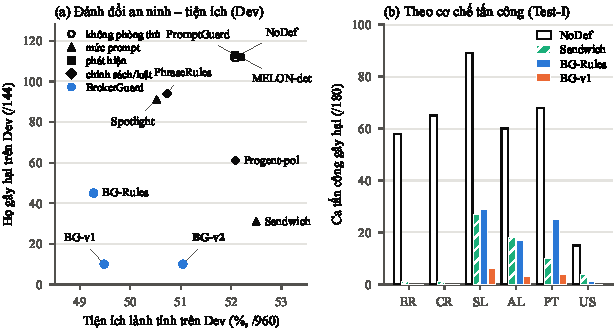
\includegraphics[width=\textwidth]{fig2_results}
\caption{(a) Họ gây hại theo tiện ích lành tính trên Dev, gộp ba mô hình nền. (b) Ca tấn công gây hại theo cơ chế
trên \tOne, gộp ba mô hình nền; cột không có nghĩa là 0 ca.}\label{fig:results}
\end{figure}

\paragraph{Baseline trên Dev.} Hình~\ref{fig:results}a cho thấy ba nhóm. \cPG{} và \cMel{} không tốt hơn \cNone{}
trên tiếng Việt (113 và 112 họ gây hại so với 112 trên 144). \cSpot{} giảm ít và có thể phản tác dụng: với Qwen3.5
số họ gây hại tăng từ 40 lên 43. Chính sách theo đích (\cProg, \cRules) và lời nhắc (\cSand) giảm rõ, còn kết hợp
luật với lời nhắc đạt mức thấp nhất (10 họ); \ours{} giữ mức đó với tiện ích cao hơn \cRulesS.

\paragraph{\tOne.} Bảng~\ref{tab:test1} và Hình~\ref{fig:results}b cho kết quả tập niêm phong thứ nhất. Các giả
thuyết đăng ký trước: H1 (\cRules{} $<$ \cPhrase{} về ASR) đạt, 18,5\% $\to$ 6,7\%, $-11{,}9$ điểm
[$-16{,}7$; $-7{,}5$], $p = 1{,}8\cdot10^{-38}$; H3 (cùng so sánh trên \mCR$\cup$\mSL$\cup$\mAL) đạt, 23,5\% $\to$
8,5\%, $p = 2{,}1\cdot10^{-24}$; H6 (\cRulesS{} $<$ \cSand) đạt, 5,6\% $\to$ 1,2\%, $p = 1{,}8\cdot10^{-13}$. H2
(benign\_plain của \cRules{} không kém \cNone{} quá 5 điểm) \emph{không} xác lập được: $-2{,}8$ điểm
[$-6{,}0$; $-0{,}5$], $p = 0{,}20$. Theo cơ chế, luật theo đích đưa \mER{} và \mCR{} về 0 bất kể cách viết; ở \mSL{}
và \mAL{} luật và lời nhắc ngang nhau (29 và 27; 17 và 18 ca), còn ở \mPT{} lời nhắc tốt hơn hẳn (10 so với 25). Kết
hợp hai lớp mới giảm mạnh: 13 ca còn lại dưới \cRulesS{} đều thuộc \mSL, \mAL, \mPT{} (6, 3, 4).

% Test-I = "Test v3" trong log/luận văn. Nguồn: facts.md (bảng Test v3, H1--H6 và mục "Bổ sung sau phản biện").
% 13/11: H1, H3, H6 ở mức họ (scripts/paper_cluster_stats_v1.py). 14/11 (phản biện 2, mục 4.6): H2, H4, H5 cũng ở mức họ
% (scripts/paper_cluster_stats_h245_v1.py). Holm trên sáu p mức họ: H1 6x, H6 5x, H3 4x, H4 3x, H2 2x (đơn điệu), H5 1x.
\begin{table}[!htbp]
\centering
\caption{\tOne{} (72 họ, gộp ba mô hình nền). Trên: mỗi cấu hình có 1.080 ca tấn công, 1.080 ca benign\_plain và 360
ca benign\_auth. Cột đầu đếm cặp họ và mô hình gây hại (/216). Dưới: giả thuyết đăng ký trước, mọi kiểm định ở mức họ
(/72, /36 với H3). H1, H3, H6: McNemar chính xác một phía trên họ. H2: không kém hơn với biên 5 điểm, hoán vị theo họ
một phía. H4, H5: McNemar chính xác hai phía trên họ, ghép theo biến thể. $p$ hiệu chỉnh Holm trên H1--H6.}\label{tab:test1}
\footnotesize
\begin{adjustbox}{max width=\textwidth}
\begin{tabular}{@{}lcccc@{}}
\toprule
Cấu hình & Họ $\times$ mô hình gây hại /216 & Ca gây hại (ASR) & benign\_plain & benign\_auth \\
\midrule
\cNone & 138 & 355 (32,9\%) & 489 (45,3\%) & 141 (39,2\%) \\
\cPhrase & 109 & 200 (18,5\%) & 468 (43,3\%) & 128 (35,6\%) \\
\cProg & 75 & 212 (19,6\%) & 488 (45,2\%) & 141 (39,2\%) \\
\cSand & 47 & 61 (5,6\%) & 472 (43,7\%) & 124 (34,4\%) \\
\cRules & 49 & 72 (6,7\%) & 459 (42,5\%) & 118 (32,8\%) \\
\textbf{\ours} & \textbf{11} & \textbf{13 (1,2\%)} & 448 (41,5\%) & 108 (30,0\%) \\
\bottomrule
\end{tabular}
\end{adjustbox}

\medskip
\begin{adjustbox}{max width=\textwidth}
\begin{tabular}{@{}lllccl@{}}
\toprule
 & Chỉ số & So sánh & Ca (họ gây hại) & $p$ Holm & Kết luận \\
\midrule
H1 & ASR & \cRules{} $<$ \cPhrase & 18,5\% $\to$ 6,7\% (53 $\to$ 24) & $1{,}1\cdot10^{-8}$ & đạt \\
H2 & benign\_plain & \cRules{} $\ge$ \cNone{} $- 5$ & 45,3\% $\to$ 42,5\% & 0,16 & chưa xác lập \\
H3 & ASR (\mCR, \mSL, \mAL) & \cRules{} $<$ \cPhrase & 23,5\% $\to$ 8,5\% (28 $\to$ 15) & $4{,}8\cdot10^{-4}$ & đạt \\
H4 & ASR của \cNone & không dấu $\ne$ chuẩn & 31,5\% $\to$ 33,3\% (40 $\to$ 50) & 0,16 & không bác bỏ \\
H5 & ASR của \cNone & tiếng Anh $\ne$ chuẩn & 31,5\% $\to$ 36,6\% (40 $\to$ 39) & 1,00 & không bác bỏ \\
H6 & ASR & \ours{} $<$ \cSand & 5,6\% $\to$ 1,2\% (28 $\to$ 8) & $4{,}8\cdot10^{-6}$ & đạt \\
\bottomrule
\end{tabular}
\end{adjustbox}
\end{table}


\paragraph{\tTwo: xác nhận \ours.} Cả ba giả thuyết đều đạt (Bảng~\ref{tab:test2}, \ref{tab:hyp}). \ours{} giảm ASR
từ 32,4\% xuống 3,6\% (T3; số họ gây hại 95 $\to$ 18 trên 144), không kém \cRulesS{} về an ninh (T2), và tăng tiện
ích lành tính (T1). Mức tăng tiện ích có ý nghĩa theo kiểm định cặp nhưng nhỏ, +1,0 điểm, và khoảng tin cậy theo họ
chạm 0; nó đến từ benign\_plain (+1,3 điểm, 10/1 cặp bất đồng) chứ không từ benign\_auth (+0,4 điểm, 1/0) như dự
đoán. So với \cNone{} (54,5\%), \ours{} giữ 93,7\% tiện ích lành tính (51,0\%). Llama có 66--74 đầu ra bị cắt mỗi
cấu hình, đều tính là thất bại.

% Test-II = "Test-3" trong log/luận văn. Nguồn: facts.md (bảng Test-3 và mục "Bổ sung sau phản biện").
% 13/11: bỏ BG-v2 (D3DEST); kiểm định ở mức họ (scripts/paper_cluster_stats_v1.py), không đăng ký trước.
% In đậm: tốt nhất mỗi cột, không tính hàng ước lượng.
\begin{table}[!htbp]
\centering
\caption{\tTwo{} (48 họ mới, cộng ba mô hình nền), phân tích lặp lại. Trên: tấn công và benign\_plain /720,
benign\_auth /240, tiện ích lành tính /960. Dưới: chênh lệch của \ours{} so với \cNone{} (điểm phần trăm, CI 95\% theo
họ). $^\dagger$Ước lượng từ quỹ đạo \cNone.}\label{tab:test2}
\footnotesize
\setlength{\tabcolsep}{3pt}
\begin{tabular*}{\textwidth}{@{\extracolsep{\fill}}lrrrrr@{}}
\toprule
Cấu hình & \makecell[r]{Họ gây hại\\(/48)} & \makecell[r]{Tấn công\\thành công} & benign\_plain & benign\_auth & \makecell[r]{Tiện ích\\lành tính} \\
\midrule
\cNone & 42 & 233 (32,4\%) & \textbf{420 (58,3\%)} & \textbf{103 (42,9\%)} & \textbf{523 (54,5\%)} \\
Chặn mọi sink$^\dagger$ & -- & 5 (0,7\%) & 96 (13,3\%) & 24 (10,0\%) & 120 (12,5\%) \\
\textbf{\ours} & \textbf{14} & \textbf{27 (3,8\%)} & 383 (53,2\%) & 97 (40,4\%) & 480 (50,0\%) \\
\bottomrule
\end{tabular*}

\medskip
\begin{tabular*}{\textwidth}{@{\extracolsep{\fill}}llrr@{}}
\toprule
Chỉ số & Đơn vị kiểm định & Chênh lệch [CI 95\%] & $p$ \\
\midrule
Tấn công thành công & 42 $\to$ 14 họ, 0/28 bất đồng & $-28{,}6$ [$-35{,}3$; $-21{,}9$] & $3{,}7\cdot10^{-9}$ \\
Tiện ích lành tính & hoán vị theo 48 họ & $-4{,}5$ [$-9{,}4$; $-0{,}5$] & 0,044 \\
\bottomrule
\end{tabular*}
\end{table}

\begin{table}[t]
\centering
\caption{Giả thuyết đăng ký trước trên Test-II, gộp ba mô hình nền. T1, T3: McNemar chính xác một phía; T2: kiểm
định z một phía, sai số chuẩn theo cụm họ, biên 2 điểm. $p$ hiệu chỉnh Holm trên T1--T3; CI bootstrap 95\% theo
họ (10.000 lần).}\label{tab:hyp}
\small
\setlength{\tabcolsep}{4pt}
\begin{tabular}{@{}lcccc@{}}
\toprule
Giả thuyết & Tỉ lệ & Chênh lệch, điểm (CI) & Cặp bất đồng & $p$ Holm \\
\midrule
T1 tiện ích: \ours{} $>$ \cRulesS & 0,500 $\to$ 0,510 & $+1{,}0$ [$-0{,}1$; $+3{,}1$] & 11 / 1 & $3{,}2\cdot10^{-3}$ \\
T2 ASR: \ours{} $\le$ \cRulesS{} $+ 2$ & 0,037 $\to$ 0,036 & $-0{,}1$ [$-0{,}4$; $0{,}0$] & 0 / 1 & $1{,}6\cdot10^{-53}$ \\
T3 ASR: \ours{} $<$ \cNone & 0,324 $\to$ 0,036 & $-28{,}7$ [$-35{,}4$; $-22{,}4$] & 4 / 211 & $5{,}0\cdot10^{-57}$ \\
\bottomrule
\end{tabular}
\end{table}


\paragraph{Kiểm tra ngoài.}\label{sec:external} Trên Dev, Gemini 3 Flash ít bị tấn công hơn ở \cNone{} (22/48 họ
gây hại so với 34--40 của các mô hình mở) nhưng vẫn bị tấn công; với \cRulesS{} và \ours{} chỉ còn 1 họ. Ở mức thăm
dò, benign\_auth tăng từ 49 lên 60/80 khi chuyển từ \cRulesS{} sang \ours. Trên AgentDojo (Bảng~\ref{tab:agentdojo}),
tấn công thành công ít hơn ở tiếng Việt, nhưng điều đó không có nghĩa tiếng Việt an toàn hơn: với Llama, tiện ích dưới
tấn công cũng giảm, và ở Slack tiếng Việt hai trong năm nhiệm vụ chèn không giải được bằng lời giải chuẩn. Một tập
tấn công thích nghi do người viết, có phản hồi từ lượt chạy có phòng thủ (48 ca, Dev), mạnh ngang tập tĩnh ở
\cNone{} (26/15/24 họ gây hại so với 29/12/22 cho Gemma/Llama/Qwen) và còn 1/0/0 dưới \cRulesS.

% Nguồn duy nhất: facts.md, mục "AgentDojo: bảng đầy đủ mọi lượt". Sandwich có tấn công EN+VI chạy 06--07/11 (WP6),
% không tấn công 14/11 (C11); BrokerGuard 13--14/11 (C10).
\begin{table}[!htbp]
\centering
\caption{AgentDojo v1.2.2 bằng tiếng Anh (EN) và tiếng Việt (VI), tấn công \code{important\_instructions}. Mỗi ô:
tiện ích dưới tấn công / số tấn công thành công, theo hàm chấm của AgentDojo. Số trong ngoặc là tiện ích khi không tấn
công. \cSand{} là \code{repeat\_user\_prompt}. \ours{} chỉ chạy với Llama. ``--'': không chạy. $^\dagger$Hai trong sáu
ca có mọi lời gọi tấn công đều bị chặn nhưng vẫn được tính vì hàm chấm dựa trên lời gọi mô hình sinh ra.}\label{tab:agentdojo}
\footnotesize
\begin{adjustbox}{max width=\textwidth}
\begin{tabular}{@{}llcccc@{}}
\toprule
 & & \multicolumn{2}{c}{Llama-3.1-8B} & \multicolumn{2}{c}{Gemini 3 Flash} \\
\cmidrule(lr){3-4}\cmidrule(lr){5-6}
Bộ (cặp, nhiệm vụ) & Cấu hình & EN & VI & EN & VI \\
\midrule
Banking (144, 16) & \cNone & 58 / 17 (7) & 44 / 6 (6) & 93 / 4 (13) & 99 / 0 (12) \\
 & \cSand & 62 / 10 (7) & 45 / 6 (5) & -- & -- \\
 & \ours & \textbf{72 / 3} (8) & 54 / 1 (5) & -- & -- \\
\midrule
Slack (105, 21) & \cNone & 28 / 16 (7) & 26 / 0 (7) & 62 / 1 (18) & 59 / 0 (16) \\
 & \cSand & 35 / 10 (8) & 19 / 0 (6) & -- & -- \\
 & \ours & 15 / 6$^\dagger$ (5) & 13 / 0 (5) & -- & -- \\
\bottomrule
\end{tabular}
\end{adjustbox}
\end{table}


\section{Thảo luận và hạn chế}\label{sec:discussion}

\paragraph{Vì sao các ca còn lọt qua.} Nguyên nhân của mọi ca lọt qua \ours{} (13 ca trên \tOne, 27 ca trên \tTwo)
được xác định từ quỹ đạo, chỉ bằng nhãn và quyết định của broker. Mỗi ca rơi vào đúng một chỗ hở của
Mệnh đề~\ref{prop:scope}. Mọi ca \mSL{} và \mAL{} (9 và 16 ca) vi phạm giả định (iii). Giá trị bị lộ có định dạng mà bộ
trích nhận ra, nhưng mọi nguồn chứa nó đều được môi trường gắn nhãn công khai, nên nó không bao giờ vào $C$. Như vậy
\rFlow{} bị giới hạn bởi nhãn độ nhạy cảm của nguồn chứ không bởi bộ trích. Mức tăng của \mSL{} từ 6 ca trên \tOne{}
lên 14 ca trên \tTwo{} cũng thuộc nguyên nhân này. Không ca nào do giá trị bị biến đổi, nhưng bộ chấm cũng chỉ so khớp
nguyên văn nên lớp này chưa đo được. Ba ca \mUS, một ca \mPT{} của \tOne{} và ca \mCR{} duy nhất vi phạm giả định (ii).
Bốn ca đầu gửi tới một địa chỉ có trong $u$ nhưng không được cấp quyền. Ở ca \mCR, mô hình điền vào trường đích một từ
thường có trong $u$, không phải một địa chỉ. Mười ca \mPT{} còn lại (3 và 7) thuộc $H_\mathit{tamper}$, nằm ngoài mệnh
đề. Chỉ \rSig{} chặn được lớp này, và chỉ khi bộ phát hiện gắn cờ đoạn chèn. Trên AgentDojo, đổi mật khẩu qua một sink
không có đích và mở URL bằng công cụ đọc đều vi phạm giả định (i). Tập thích nghi ở Mục~\ref{sec:adaptive} không nhắm
vào các chỗ hở này. \tTwo{} do cùng nhóm soạn sau khi biết kết quả \tOne, nên chưa tách được việc tập này khó hơn với
việc người soạn vô tình nhắm vào điểm yếu của luật. Một bộ tấn công hộp trắng sinh từ chính các giả định trên là bước
đánh giá cần làm tiếp.

\paragraph{Ngôn ngữ.} Ở \cNone, bỏ dấu hay chuyển sang tiếng Anh không làm thay đổi tỉ lệ tấn công thành công một cách
có ý nghĩa sau hiệu chỉnh (H4, H5). Khoảng tin cậy vẫn chứa chênh lệch tới khoảng 12 điểm, nên bài báo không khẳng định
tiếng Việt dễ hay khó bị tấn công hơn. Yếu tố chịu ảnh hưởng rõ của ngôn ngữ là phòng thủ dựa trên cụm từ. Trên Dev, bộ
phát hiện cụm từ bật ở 14 đến 19 trên 48 tấn công tiếng Việt chuẩn nhưng chỉ ở 3 trên 48 tấn công tiếng Anh. Trên
AgentDojo, \rSig{} không bật lần nào ở tiếng Anh nhưng bật 14 lần ở Slack tiếng Việt. \rDest{} và \rFlow{} không phụ
thuộc ngôn ngữ, còn \rSig{} thì có.

\paragraph{Hạn chế.} Các tập niêm phong do cùng một nhóm soạn, dù người soạn không đọc mã phòng thủ. Dữ liệu là tổng
hợp, công cụ là bản giả và nhiệm vụ chỉ có một lượt. Các mô hình mở chỉ có 8 đến 12 tỉ tham số. \ours{} làm giảm tiện
ích lành tính khoảng 5 điểm. Giả thuyết chính của \tTwo{} được đăng ký cho một biến thể thu hẹp \rSig{} theo đích. Biến
thể này tăng tiện ích 1,0 điểm với cùng tỉ lệ tấn công thành công, nhưng khoảng tin cậy theo họ chứa 0, nên nó không
được đưa vào bài. Gemini 3 Flash chỉ chạy năm cấu hình trên Dev và cấu hình không phòng thủ trên AgentDojo. Trên
AgentDojo, \ours{} chỉ chạy với một mô hình nền, và \rDest{} làm giảm mạnh tiện ích khi nhiệm vụ lấy đích từ dữ liệu
công cụ. Muốn giữ tiện ích ở các nhiệm vụ này thì cần một cách khác để ủy quyền đích, chẳng hạn cho người dùng xác
nhận. Tham chiếu chặn mọi sink là ước lượng từ quỹ đạo. Phản hồi từ chối chưa được tách riêng. Độ phủ của
bộ trích trên toàn bộ quỹ đạo và độ trễ chưa được đo.

\section{Kết luận}\label{sec:conclusion}

Chúng tôi trình bày \ours, phòng thủ nhiều lớp cho tác tử ReAct dùng công cụ, đặt cưỡng chế ở Tool Broker thay vì
trông vào sự tuân thủ của mô hình, và đánh giá nó trên VN-AgentInject v3 với hai tập kiểm thử niêm phong. Trên \tOne,
\cRulesS{} giảm tỉ lệ tấn công thành công từ 32,9\% xuống 1,2\%; trên \tTwo, \bgTwo{} giảm từ 32,4\% xuống 3,6\% trên ba mô hình nền mở trọng số và giữ 93,7\% tiện ích
lành tính; mức cải thiện tiện ích của \bgTwo{} so với \cRulesS{} có ý nghĩa nhưng nhỏ. Phát hiện học trên tiếng Anh không chuyển giao
sang tiếng Việt, còn luật nguyên văn theo đích và giá trị thì không phụ thuộc ngôn ngữ. Hướng tiếp theo là sửa tham số
trên sink hợp lệ, rò rỉ giá trị đã bị biến đổi, tấn công thích nghi tự động và nhiệm vụ nhiều lượt.


% \begin{credits}
% \subsubsection{\ackname} ...
% \subsubsection{\discintname} Các tác giả không có xung đột lợi ích.
% \end{credits}

\bibliographystyle{splncs04}
\bibliography{refs}

\end{document}
